\parx
Figure \ref{fig:cn_debug} shows Terminal window can be toggled open by the keyboard
shortcut \textbf{ctrl + shift + t}. The Terminal displays messages for the
status of the visual code. The Terminal can display warning (yellow colored)
and error (red colored) messages for debugging.

\begin{figure}[H]
	\centering
	\captionsetup{justification=centering}
	\captionsetup[figure]{list=yes}
	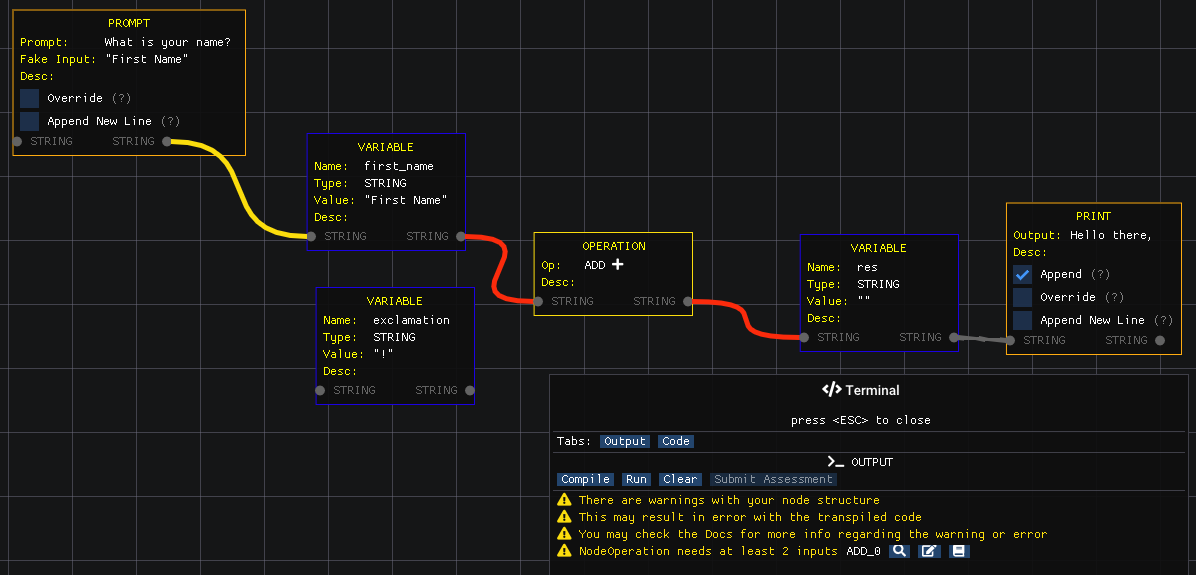
\includegraphics[width=\linewidth]{media/sc_debug.png}
	\caption[Screenshot of Terminal and Debug in CodeNect]{Screenshot of Terminal and Debug in CodeNect}
	\label{fig:cn_debug}
\end{figure}

\parx
Figure \ref{fig:cn_transpiled_code} shows code tab in the Terminal window that
displays the transpiled visual code into the C programming language. The code
can be copied into clipboard or save into a separate file.

\begin{figure}[H]
	\centering
	\captionsetup{justification=centering}
	\captionsetup[figure]{list=yes}
	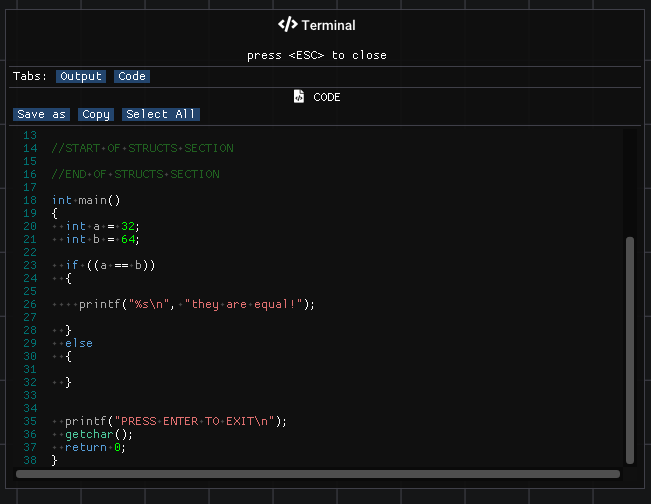
\includegraphics[width=\linewidth]{media/sc_transpiled_code.png}
	\caption[Screenshot of Transpiled Code Tab in Terminal]{Screenshot of Transpiled Code Tab in Terminal}
	\label{fig:cn_transpiled_code}
\end{figure}

\parx
Figure \ref{fig:cn_run} shows the transpiled code executed and running natively in the
command prompt (for Windows) or terminal (for Linux).

\begin{figure}[H]
	\centering
	\captionsetup{justification=centering}
	\captionsetup[figure]{list=yes}
	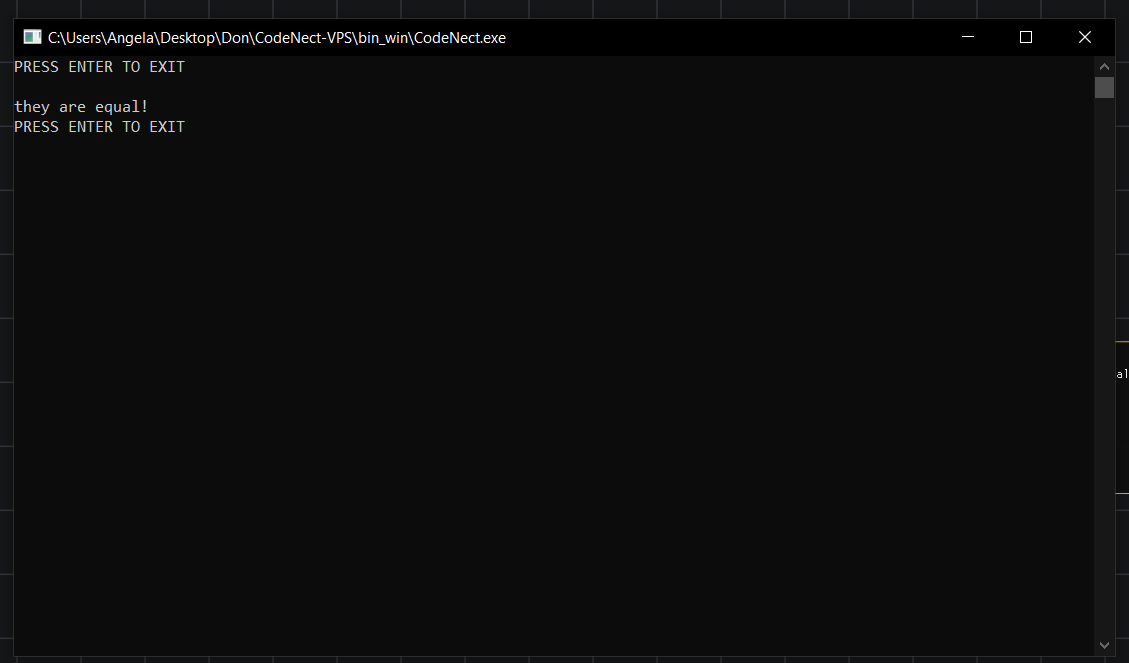
\includegraphics[width=\linewidth]{media/sc_run.png}
	\caption[Screenshot of Running Transpiled Code]{Screenshot of Running Transpiled Code}
	\label{fig:cn_run}
\end{figure}
